\subsection{Feature Diagrams}\label{ch:feature-diagram}

\begin{figure}[h]
    \centering
    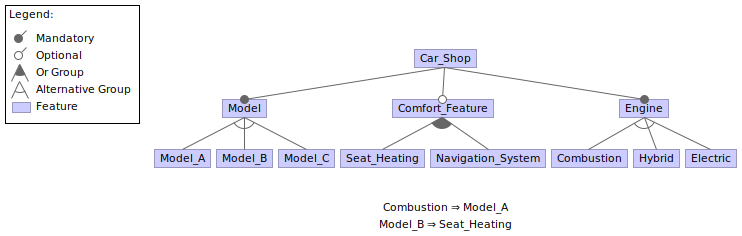
\includegraphics[scale=0.55]{gfx/Car_Shop.png}
    \caption{A feature diagram of a car dealership.}
    \label{fig:car}
\end{figure}

%What is a feature diagram and relation between features
A feature diagram is conceptually built as a tree where each node of the tree represents a feature, 
for which edge between a parent node and a child usually implies that the parent is a more general concept and the child a specialization. 
So, the further we descend in the tree, the more specialized the feature gets; with regard to its subtree.

%Feature diagram example
\autoref{fig:car} is an example for a feature diagram that depicts the structure of a car dealership. We see that the root
node \textit{car\_shop} represents the overall system. As we descend we look at the child nodes of the
\textit{Engine} feature, we can see concrete engine types, such as \textit{Combustion}, \textit{Hybrid}, and \textit{Electric}.

%Concrete and abstract feature with example
We differentiate between two types of feature nodes: \emph{abstract} and \emph{concrete} feature. 
Abstract features are used to structure the diagram, as such they not correspond to a concrete implementation.
In contrast, concrete features reflect variability inside the system, where a concrete feature is bound to an implementation artifact~\cite{Feature-Oriented-Software-Product-Lines}.

In \autoref{fig:car}, the feature \textit{Engine} is considered an abstract feature since it does not implement anything and 
is only used to give the feature diagram more structure by grouping all kinds of engines a car can possess and signaling 
the user that he must select a specific engine.
The specific engines, like \textit{Combustion} are concrete features that implement specific types of functionality.

%Mandatory and optional feature
Each feature contains a graphical notation indicating whether the feature is mandatory or optional. 
If the feature is mandatory, it is indicated with a black bubble any if it is optional, it is displayed with an empty bubble~\cite{Feature-Oriented-Software-Product-Lines-Feature-models}. 
In \autoref{fig:car}, we can see that \textit{Engine} and \textit{Model} are mandatory features, which make sense given that they are are necessary for any car 
but \textit{Comfort\_Feature} is optional and not necessary for a car to function.

%Alternative and choice groups
In addition to mandatory and optional features, there are alternative and choice groups. 
A parent can have one of the groups the alternative group is marked with an empty half circle and the choice group with a filled circle. 
When we use a choice group, one feature must be selected, but others can also be selected. Therefore, the choice group corresponds to the logical \textit{or} operator. 
In an alternative group, we can select only one feature; the configuration is invalid if more than one feature is selected~\cite{Feature-Oriented-Software-Product-Lines-Feature-models}. 
In \autoref{fig:car}, we see that \textit{Engine} has an alternative group, since each car can only contain one \textit{Engine}, 
whereas it makes sense that \textit{Comfort\_Feature} contains a choice group: one can have a navigation system and seat heating in a car without conflict.

%Constraints
A feature diagram may contain various constraints that need to be satisfied, defined as boolean algebra. In \autoref{fig:car}, we see two constraints, 
$Combustion \implies Model\_A$ and $Model\_B \implies Seat\_Heating$. The reason for such constraints could be that \textit{Model\_B} 
is a luxury model that only gets shipped with seat heating.

%Propositional formula , why useful
We use a feature model to check whether a configuration 
is valid, which is particularly useful if we want to sample or enumerate all valid configurations~\cite{Feature-Oriented-Software-Product-Lines-Feature-models}. 